\documentclass[10pt]{article}

\usepackage{listings}
\usepackage[utf8]{inputenc}
\usepackage{color}
\usepackage{textcomp}
\usepackage{a4wide}
\usepackage{graphicx}

\definecolor{listinggray}{gray}{0.9}
\definecolor{lbcolor}{rgb}{0.99,0.99,0.99}
\lstset{
	backgroundcolor=\color{lbcolor},
	tabsize=2,
	rulecolor=,
	language=Matlab,
	basicstyle=\footnotesize,
	upquote=true,
	aboveskip={0.8\baselineskip},
	columns=fixed,
	showstringspaces=false,
	extendedchars=true,
	breaklines=true,
	prebreak = \raisebox{0ex}[0ex][0ex]{\ensuremath{\hookleftarrow}},
	frame=single,
	showtabs=false,
	showspaces=false,
	showstringspaces=false,
	identifierstyle=\ttfamily,
	keywordstyle=\color[rgb]{0,0,1},
	commentstyle=\color[rgb]{0.133,0.545,0.133},
	stringstyle=\color[rgb]{0.627,0.126,0.941},
}



\title{COSICAF muanual}
\author{Gregoire de Izarra}


\begin{document}
	\maketitle
	
	\tableofcontents
	\newpage
	\section{What COSICAF does}
	
	COSICAF is a tool for simulating nuclear instrumentation. It was developped with
	fission chamber in mind but might be adapted to any other gaseous detector.
	Its main goal is to estimate gaseous detector output signal by simulating all
	the physical processes involved in the neutron detection.
	The code is mainly for educational purpose but is valuable as well for research
	since it provides correct quantitative estimations.
	
	COSICAF is constructed to provide two levels of simulation. The first one is low
	level, it gives access to basic data and models to make students build their own
	Monte Carlo simulation code easily. The second level of simulation provides
	advanced  features like geometry description, particle tracking, electrostatic
	and induced current computation. 
	
	The software is written in Octave/Matlab langage to provide easy data manipulation
	and plots at the cost of low computational efficiency. 
	
	\section{Installation}
	
	COSICAF was tested with various version of Octave and Matlab. It was reported to work with:
	
	\begin{itemize}
		\item Octave 4.4 branch.
		\item Octave 5 branch.
		\item Matlab 2013b.
		\item Matlab 2016a.
		\item Matlab 2017a.  
	\end{itemize}
	
	 For some features like 3d display of the geometry, Octave version 4.4.1  at least is needed.
	 To install COSICAF, copy the directory on the hard drive of your computer. Add the COSICAF directory to the path of your Octave or Matlab installation. With Octave it is done by writing those lines in the octave command prompt:
	 
	 \begin{lstlisting}
	 addpath 'C:/MYPATH/COSICAF'
	 savepath	 
	 \end{lstlisting}
	 
	 Two C++ versions of an electrostatic solver are included with cosicaf. They are written specifically for octave and should be used to make oct files. To build the function, go to the cosicaf directory and write:
	 
	 \begin{lstlisting}
	 mkoctfile -O3 mcVspecial.cpp
	 mkoctfile -O3 mcV.cpp
	 \end{lstlisting}
	 
	 No native version of the electrostatic solver is available for matlab. Instead, the script version, much slower, can be used.
	 Once this is done, it is possible to use the COSICAF code to simulate gaseous detectors.
	 
	
%	\section{How the code works}
%	
%	COSICAF is a modular fission chamber simulation code. It gives access to basic models and also to high level features like particles tracking, geometry electrostatic computation etc.
%	
%	    The main goal of the code is to be used for educational purpose. To reduce the needed amount of data, all the models are mostly based on fitted function. The amount of data needed is low enough to consider hand computation or a port of the simulation on pocket calculator.
%	    
%	    Each physical process is considered independent from the other one involved in signal generation. Because of that approximation, the effect of charges spaces related to high neutron flux cannot be captured. Heavy ions are travelling instantaneously to uncouple signal generation from 
	
	\section{Data used in cosicaf, and how to add additionnal models}
	The fits used in COSICAF are coming from multiple sources:
	
	\begin{itemize}
		\item For heavy ion moderation laws: an CEA code with a first order PRAL implementation and SRIM.
		\item For 'electronic' energy loss, the data is coming from SRIM.
		\item For electron drift velocities: raw data is coming from 'Gaseous electronics: theory and practice' by G.G. Raju, from papers on argon/nitrogen mixture plasma by Haddad, and from Bolsig sofwtare.
		\item For the first Townsend coefficient, data from Kruithof (1940 physica 7) is used. No implementation of avalanche is implemented in COSICAF but fits are available.
	\end{itemize}
	
	The fits were done with Gnuplot. The coefficients are stored in \lstinline{.dat} files inside the main directory of COSICAF.
	All the data is retrieve with keywords. It is possible to define some new keywords if different gas mixtures are needed or if new heavy ions must be used. Be sure to use the same keyword for the gas mixture and for the heavy ion in all the data files. Raw data used for COSICAF are stored in the \lstinline{raw_data} directory for code improvement and traceability.
	
	\subsection{Moderation laws}
	The models used by cosicaf for moderation laws are the following:
	
	\begin{equation}
	E(x)=E_{0}\left(1-\frac{x}{R_{E_{0}}}\right)^{n},
	\label{eq:simple_sp}
	\end{equation}

	\begin{equation}
	E(x)=E_{0}\left[a\left(1-x/R_{E_0}\right)+b\left(1-x/R_{E_0}\right)^2+c\left(1-x/R_{E_0}\right)^3+d\left(1-x/R_{E_0}\right)^4+e\left(1-x/R_{E_0}\right)^5\right]
	\end{equation}
	
	$E_{0}$ is the initial energy of the heavy ion (in MeV) $R_{E_{0}}$ the range (in mg/cm$^{2}$), $x$ the travelled distance. In equation \ref{eq:simple_sp}, $n$ a semi empirical parameter obtained through a fit while for the polynomial approximation, the fitted  parameters are $a$, $b$ $c$, $d$, $e$.
	

	
	Here is an extract of the moderation law datafile:
	 
	 \begin{lstlisting}
	 #* Medium, particle, E0(MeV), Range (mg/cm^2), Pow. law,a,b,c,d,e
	 #*************************************************************
	He	hffU5	68.5	1.7667	1.9474	0.36372	-0.24186	1.1692	-0.13061	-0.16050
	 \end{lstlisting}
	 we defined a gas mixture called \lstinline{He}, this keyword will be used afterward during simulation script and geometry definition. The moderation law described here is the one uranium 235 light fission fragment.
	 All datafiles contain a header with the data organisation and the needed units, it is mandatory to follow it in order to include additional models. Here, the datafile contain the initial energy of the projectile, the range in $mg/cm^{2}$, a parameter for a power law  approximation of moderation law, and parameters for the five order polynomial approximation.
	 When deriving new moderation laws, be careful to have monotonous function since inverse moderation law use dichotomy method to make correspond a travelled distance to an energy loss.
	 
	 \subsection{Electron drift velocity}
  Electron drift velocity is described by fits on a set of reduced electric field intervals in order to capture correctly all the possible drift velocities changes.
  Three different functions are used for fitting:
  \begin{itemize}
  	\item 0) $f(x)=a.x^b$.
  	\item 1) $f(x)=a.x+b.x^2+c.x^3+d$.
  	\item 2) $f(x)=a.(1-exp(b.(x)^c))$
  \end{itemize}
   
   Each function is related to an index to make the routine aware on how to use fit parameters. An example of the electron drift velocity is shown below:
   
   \begin{lstlisting}
   #********ELECTRON DRIFT_VELOCITY *****************************
   #*-g. de Izarra, CEA Cadarache-------------------------------- 
   #* Give the drift velocity in 10^3 (m/s)
   #* fit type :
   #* 0-> f(x)=a*x**b 
   #* 1-> f(x)=a*x+b*x**2+c*x**3+d 
   #* 2->f(x)=a*(1-exp(b*(x)**c)) 
   #* Medium, fit_type, low bound (Td), high bound (td), a,b,c,d
   #*************************************************************
   He  0	0.02	0.2	5.94741	0.624701	0	0
   He  0	0.2	7	4.81119	0.560496	0	0
   He  1	7	200	2.27587	0.00722098	-2.62E-05	0
   \end{lstlisting}
   
	For each domain, the type of function to use for the fit, the fit domain in Tonwsend, and the fit parameters are defined. Additional data should give velocities in $10^{3}$ (m/s). The fit domain should be contiguous. 
   Once data is loaded, it is stored in a \lstinline{caf_problem} object as a cell array named \lstinline{e_drift_data}.
   
   
   \subsection{Ion drift velocity}
   
   Ion drift velocity is obtained by using the frost semi-empirical law. The parameters used in COSICAF were obtained by Goyatina and Maiorov, they are available in the paper "Approximation of the characteristics ion drift in parent gas", Plasma Physics Report 43:75-17. It is possible to increase the database by fitting the frost law on other experimental or theoretical data. The datafile format is as it follows:
   
   \begin{lstlisting}
   #********ION DRIFT_VELOCITY *****************************
   #*-g. de Izarra, CEA Cadarache-------------------------------- 
   #* The ion drift velocity are coming from the paper: 
   #* Approximation of the characteristics of Ion Drift in Parent Gas
   #* by R. I. Golyatina and S. A. Mairov
   #* Plasma Physics reports vol 42 n 1
   #* The file contains coefficients depending of the temperature
   #* for the Frost semi-empirical formula which is:
   #*
   #* v=a(1+b*E/N)^{-0.5}*E/N with E/N in td and v in (cm/s)
   #*------------------------------------------------------------
   #*Ion	T(K) a(cm/(s.Td)) 1/b(Td) T a b ...  
   #*************************************************************
   He	4.2	5632	17	77	4162	33	300	2774	85	1000	1787	210	2000	1374	410
   Ne	4.2	1888	35	77	1605	45	300	1117	103	1000	771		240	2000	591		450
   \end{lstlisting}
   Each line correspond to a specific material. The keyword linked to the material starts the line. Then, block consisting of temperature, $a$ and $b$ two parameters for the Frost law are written. 
   The routine in charge of drift velocity computation uses linear interpolation between temperature, due to the loading routine \lstinline{load_ion_drift_velocity}, at least five temperatures must be written for each gas. The loading routine should be improved to make the file format more flexible.
   
   
   \subsection{Mean energy needed to produce ion pair}
   
   The $W$ value were obtained from ICRU reports and from Kushner's papers on electron beam plasma. The datafile is as simple as possible. Each line contains the name of the material and the corresponding W in eV.
   During charged meta-particles transport, W data is used to see if the electron and ions can drift in the related material. If not, particles are killed. Care must be taken to include additional data, since it will affect the particle drift. 
   
   
	\section{Geometry description}
	
	All the geometry in COSICAF is built from cylinders or cylinder shells.
	No binary operations are allowed between cylinders, in addition, they are all parallel to the z axis. However, inclusion relation could be described thank to a inclusion index: low inclusion index volumes enclose volumes with higher indexes. Each volume has a material and a density defined. Some special volumes also have no collision with heavy ion, can emit particles or are able to stop them directly.
	
	The geometry is defined in a special text file wich has the following organisation:
	
	\begin{lstlisting}
	#********GEOMETRY_DEFINITION********************
	#* g. de Izarra, CEA Cadarache 
	#***********************************************
	#* Header: 
	#* 
	#* Planar geometry  CFP12 like. 
	#* Test with 1 volume of gas,
	#* two electrodes.
	#* One fissile deposit with U5
	#*
	#***********************************************************************
	#ID	type	ext.rad	in.rad	height	position	mat.	densty  electrod	source particle energy emission
	#***********************************************************************
	1	bound   0.008	0	0.01	0	0	0		Ar		1.78e-3		0			0	none	0	0
	2	regular	0.005	0.001	0.005	0	0	2e-3	Ar		1.78e-4		0			0	none	0	0	
	2	regular	0.005	0	1e-6	0	0	1e-3	U3O8	9.8			0			1	lffU5 99.8	0.5
	2	no_coll	0.005	0	1e-6	0	0	1e-3	U3O8	9.8			0			1	hffU5 68.0	0.5
	2	stop   0.005	0	1e-3	0	0	0		U3O8	9.8			1			0	none	0	0
	2	stop   0.005	0	1e-3	0	0	0.009	U3O8	9.8			1			0 	none	0	0	
	\end{lstlisting}
	
	Line beginning with \lstinline{#} are comments. Each line describing the geometry starts with the inclusoin index. Then the type of volume is define. It can be \lstinline{regular} or represent the \lstinline{bound}
	 of the  simulation domain. It is also possible to define volume with no collision (\lstinline{no_coll}) or with collision strong enough to stop every projectile  (\lstinline{stop}). Then external and internal radius of cylinder shell are defined as well as its height and the location of its lower basis. Material is then defined with the related density. At last, it is specified if volume is an electrode or a source and which particle at what energy it emit.
	  
	
	\section{Tutorial : access to the basic models}
	The access to the first level of modeling is interesting to build a simulation from scratch. During practical work described in the paper XXXX, students are asked to build a simple Monte Carlo code relying on the basic COSICAF models.
	
	To use the low level models, it is necessary to define a \lstinline{caf_problem} object which contains all the method and the associated data for fission chamber simulation. Then, the data stored in .dat file located in the base directory of COSICAF must be loaded in memory:
	
	\begin{lstlisting}
	obj=caf_problem(); % caf_poblem defined
	% yet it contain no data for simulation,
	% We have to load those from .dat files.
	
	ret=obj.load_moderation_laws(); % loading moderation laws data
	% if the loading is successful, the ret value is 1.
	
	ret=load_elecEcorr(); % loads the correction to only consider
	% the electronic energy losses.
	
	ret=obj.load_molar_mass(); %molar mass of few material used 
	% in the simulation
	
	ret=obj.load_W(); %loading of the W values
	
	ret=load_ion_drift_velocity() % loads the fit parameter
	% for the Frost semi empirical model.
	
	ret=load_e_drift_velocity() % loads the electron drift
	%velocity fit parameters.
		
	\end{lstlisting}
	
	Once every data is loaded, models can be used. Here is an example of moderation law and inverse moderation law use:
	
	\begin{lstlisting}
	
	%HffU5 in Ar 0.0017 g/cm^3, Energy after 1 cm travel:
	 Epow=obj.moderation_law('Ar',0.0017,'hffU5',1e-2,'POW')
	% 4 parameters are needed. The first one is a string
	% defining the target medium, here argon. The second
	% parameter is the density of the target medium in
	% g/cm^3. The third parameter is a string which define
	% the kind of projectile, here it is a heavy U5 fission
	% fragment. At last, the final parameter is the 
	% moderation law approximation. 'POW' is a simple power
	% law which is simple enough fo analytical derivation.
	% The approximation 'POLY' also exist, it gives far better
	% results (5 order polynomial) but is more complicated for
	% comparison with hand computations.
	
	Epoly=obj.moderation_law('Ar',0.0017,'hffU5',1e-2,'POLY')
	% same as below but with polynomial approximation of 
	% modeation laws
	
	l=obj.inverse_moderation_law('Ar',0.0017,'hffU5',16.16445, 'POLY')
	%here an inverse moderation law is used to estimate the distance
	% travelled corresponding to an energy loss of 16.16445 MeV of
	% a E0 heavy ion.
	% 4 parameters are needed: the target medium, the density of the
	% target medium, the type of projectile, the energy loss
	% in MeV and the approximation.
	
	\end{lstlisting}
	Inverse moderation laws are useful for taking into account the energy already lost by the heavy ion during travel through different material.
	
   Other data like electron or ion drift velocities are available in COSICAF, they can be used in the following way: 
	
	\begin{lstlisting}
	
	Er=obj.compute_reduced_Efield(200000,'Ar',1.7e-3);
	% Compute the reduced electric field (in Td).
	% The routine takes as input: 
	% the electric field (in V/m), the material, the density in (g/cm^3)
	% This routine uses the molar masses loaded with the routine  load_molar_mass()
	
	evel=obj.e_drift_velocity('Ar',Er);
	%compute the electron drift velocity in (m/s)..
	% It take as input the name of the medium where the drift velocity
	% has to be computed and the reduced field (in Td)
	
	T=300;
	ivel=obj.ion_drift_velocity('Ar',T,Er)
	%Compute the ion drift velocity in (m/s)
	% take is input the name of the medium were the drift velocity
	% is computed, the heavy particle temperature and the reduced  E field.
	% It is assumed that the ion of interest is the signly ionised medium.
	 
	\end{lstlisting}
	
	
	
	\section{Tutorial: typical organisation of a high level simulation}
	
   Due to its modular design, COSICAF is not automatized and a few steps have to be performed to simulate the pulses of fission chambers.
   Those steps are grouped in an octave script which contains:
   \begin{itemize}
   	\item Definition of \lstinline{caf_problem}.
   	\item Loading of COSICAF data.
   	\item Loading of the geometry.
   	\item Plotting the geometry for visual sanity check.
   	\item Setting the simulation parameters: number of heavy particles to simulate, time steps, number of charged meta-particles to generate along fission fragment tracks...
   	\item Setting the electric field and the weighting fields.
   	\item Initialising heavy particles (position, energy, direction of propagation).
   	\item Propagating projectiles along the geometry.
   	\item generating fission track and the associated current pulses.
   \end{itemize}
	
	
	As for the access to the basic models, the loading of CASICAF data is done with the following script:
	
	\begin{lstlisting}
		obj=caf_problem(); % caf_poblem defined
		% yet it contain no data for simulation,
		% We have to load those from .dat files.
		
		ret=obj.load_moderation_laws(); % loading moderation laws data
		% if the loading is successful, the ret value is 1.
		
		ret=load_elecEcorr(); % loads the correction to only consider
		% the electronic energy losses.
		
		ret=obj.load_molar_mass(); %molar mass of few material used 
		% in the simulation
		
		ret=obj.load_W(); %loading of the W values
		
		ret=load_ion_drift_velocity() % loads the fit parameter
		% for the Frost semi empirical model.
		
		ret=load_e_drift_velocity() % loads the electron drift
		%velocity fit parameters.
	\end{lstlisting}
	
	
	Once the data is loaded, the geometry has to be loaded and plotted.
	
	\begin{lstlisting}
	obj.load_geometry('my_geometry.txt' ); %loading the geometry
	
	clf(); % clear figure
	
	obj.draw_geometry(); %the loaded geometry is drawn
	\end{lstlisting}
	
	If the geometry seems ok, the script can be further extended to set 
	simulation parameters. Few parameters has to be set, first the number of heavy particles to simulate. Not all the particles lead to pulses, some are stopped before entering in gas volumes. If a specific number of pulses is needed, a coarse estimation of the number of heavy particles to simulate should be done. Another important parameter is the number of charged meta-particles to produce. For each fission tracks, the code will produced two time the number of meta-particles asked, half will be ions and half electrons. A value around few hundreds is recommended and should work on most of simulations. 
	
	\begin{lstlisting}
	obj.particle_nb=5000;
	%definition of the number of particle to simulate.
	% if the geometry is complicated increase this number.
	% For statistic since not all the particles lead to current pulse.
	% The time needed to propagate heavy part is negligible
	% in front of the time needed to compute pulses.
	
	obj.charge_nb=300;
	%definition of the number of charged meta particles to generate
	\end{lstlisting}
	
	The time step and the max simulation time per pulse are critical. Due to order of magnitude difference between ion and electron drift velocities, it might be clever to tune the time step and the max simulation time for each type of charged particle and to simulate separately the ionic and the electronic signal. The time step has to be choosen carefully since it impact the error on induced current. Here is an example of parameters for electronic pulse simulation only:
	
	\begin{lstlisting}
	obj.time_step=0.01e-9; %definition of the time step
	
	obj.max_time=10e-9; %definition of the max simulation time
	\end{lstlisting}
	
	The electric field and the electrodes weighting field are included
	 in the simulation with function handles. Functions must take as parameter a three elements vector representing the position where to compute the field and return the electric field as a vector.
	 For each simulation, electric and weighting field function must be defined in a separated file. If potential computed by COSICAF are used, it is possible to encapsulate the routine \lstinline{compute_E_from_mc_V}.
	 
	 Here is an example of function defining electric field:
	 
	 \begin{lstlisting}
	 %this is stored in mpfd_E_field.m
	 function E=mpfd_E_field(pos)
	 
	 dl=0.5e-4;
	 E=obj.compute_E_from_mc_V(pos,V_E,pos_voxel_E,pos_geom_E,dl);
	 % This routine allow to derive electric field from 
	 % potential matrix computed by COSICAF.
	 end
	 \end{lstlisting}
	 
	 \begin{lstlisting}
	 %this is stored in CFUR_weighting_E.m
	 function E=CFUR_weighting_E(pos)
	 
	 % E(r)= dV/(rlog(Ro/Ri))
	 vec=[pos(1) pos(2) 0];
	 vec=vec/norm(vec);
	
	 r=sqrt(pos(1).^2+pos(2).^2); 
	 E=1/(r*log(1.25/1))*vec;
	 
	 if(r<1e-3)
	 E=[0 0 0];
	 end
	 
	 end
	 \end{lstlisting}
	 
	 In the simulation script, the electric field and the weighting field related to every electrode of interest is taken into account by writing:
	 
	  \begin{lstlisting}
	  
	  obj.elec_field=@CFUR_E %definition of the electric field.
	  %The handle on the CFUR_E routine is used.
	  
	  %weighting field for electrode are kept in memory
	  % by using cell containing handle functions.
	  
	  %let us define a single electrode of interest, we have:
	  obj.weighting_field=cell(1) % 1 cell is defined
	  obj.weighting_field{1}=@CFUR_weighting_E % the handle is stored 
	  % in the cell
	  \end{lstlisting}
	  
	  since heavy ion transport and charge track generation are uncoupled to signal computation, it is possible to change the time parameters, the electric field and the number of charged particles to generate at every moment.
	
		Since every parameter of the simulation is defined, it is now possible to start the heavy ions generation and transport. This is done with:
		
		\begin{lstlisting}
		obj.init_heavy_particles(); 
		%initiate the heavy particle, that is to say
		% it randomly compute:
		% - a travelling direction.
		% - a position.
		% - the kind of projectile if more than one source
		%   is defined. 
		% this is done in a batch on obj.particle_nb particles
		
		% the particle position and direction is available
		% in obj.particle{2,x} where x is the particle index
		% the type of heavy of heavy particle is available in
		% obj.particle{1,x}
		
		% the tracking of each particle is done with:
			
			for i=1:obj.particle_nb;
			obj.propagate_one_heavy_particle(i,'POLY');
			end
		
		\end{lstlisting}
		
		If needed, it is possible to visualize trajectories in the problem geometry by using:
		
		\begin{lstlisting}
		clf 
		i=1
		obj.draw_particle_trajectory(i);
		%draw the trajectory of the particle i
		
		%draw the geometry to locate trajectories
		obj.draw_geometry();
		\end{lstlisting}
		An example of the plot generated for 100 trajectories in a small cylindrical fission chamber is available in figure \ref{fig:100trajectoires}.
		
			\begin{figure}[!htb]
			\centering
			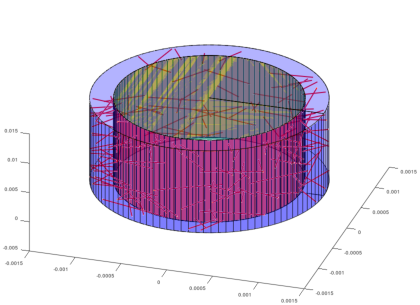
\includegraphics[scale=1.3]{100trajectoires.pdf}
			\caption{Example of a trajectory plot done by COSICAF.}   
			\label{fig:100trajectoires}
		\end{figure}
		The computation of detector pulses is done by generating electric charges along heavy ion track and by makin them move while recording the induced current on electrode. With COSICAF routine it gives:
		
		\begin{lstlisting}
		for i=1:obj.particle_nb %o throught the particles
		
		% generate charges along h ion track
		ret=obj.generate_charge_track(i,'POLY');
		%ret contains the number of charged meta particle
		% generated. If no charge is created it is empty.
		
		if(isempty(ret)==0) % if charges were created
		
		obj.kill_ions(); % we kill ions to only get
		%the electronic signal (it is possible to
		% kill electrons with kill_electrons())
		
		%go through the time step		
		for j=1:round(obj.max_time/obj.time_step) % time step for pulses computation.
		
		obj.move_charge_track([1,j]);  
		% move charges and compute induced currents on electrodes.
		end
		
		% the induced signals are stored in obj.signal array
		
		\end{lstlisting}
		
	\section{Electrostatic computation}
	
	 COSICAF contain a electrostatic solver based on random walks. Multiple versions of the algorithm are available, for octave, C++ version allows to speed up drastically the computation of the potential all along the geometry. For Matlab or if octfile compiler is not available, a .M function is accessible through a cafproblem object.
	 
	 To use the solver, it is first necessary to describe the electrostatic problem by defining all the dielectric permittivity of the volume and the boundaries conditions. This is done by using a file organised in the same way as the geometry description of the problem. Each line of the file correspond to a volume defined at the same line in the geometry file. The electrostatic file define for each volume the outer, inner upper and lower potential of each volume plus the relative dielectric permittivity. Not all the volume get potential boundary value, the absence of boundary value is represented by a \lstinline{no} key word. Since the method used is random walk, it is mandatory to use only dirichlet boundary condition. In addition the main volume must have all his boundaries defined to a correct value to prevent crashes of electrostatic solver. 
	 
	 The following example is a file used to define the electrostatic problem for a planar detector test case. The detector body is polarised, and a volume with a different permettivity value is set in the middle of the detector.
	 
	\begin{lstlisting}
	#********ELECTROSTAT_DEFINITION*********************************************
	#* g. de Izarra, CEA Cadarache 
	#***************************************************************************
	#* Header: 
	#* 
	#* This file works with a geometry definition file. 
	#* It define the quantities needed to generate a discrite mesh for
	#* solving the poisson equation.
	#* The order of the boundaries and the permitivity correspond to the order 
	#* where volume have been defined.
	#***************************************************************************
	#outerV InnerV upperV lowerV permittivity
	#***************************************************************************
	1	no	20	-20	1
	no  no  no  no  1.3
	no  no  no  no  1
	no  no  no  no  1
	no	no	no	no	1
	no	no	no	no	1
	\end{lstlisting}

	A routine of COSICAF was written to load the electrostatic data of a simulation it is: 
	\begin{lstlisting}
	obj=caf_problem(); % creation of a caf_problem object
	%...
	obj.load_geometry('mpfd_geometry_paper.txt' ); % Loading of the problem geometry
	
	obj.load_geometry_electrostat_dat('mpfd_geometry_paper_V_SOLVER.txt');% loading of the electrostatic data related to the problem geometry.
	\end{lstlisting}

    Once the geometry and the electrostatic data is loaded in memory, the geometry has to be converted into a discrete mesh. This is done by the \lstinline{convert_geom_Vmcsoler} routine.
    This routine use brenenham line algorithm and a flood and fill algorithm to build meshes with the proper boundary conditions and permittivity:
       
	\begin{lstlisting}
	[condlim,permit,pos_voxel,pos_geom]=obj.convert_geom_Vmcsolver(0.5e-4);
	% Convert the surface geometry into a one with discrete mesh. The descritisation step
	% (in meter) is the only input nedeed. The function return condlim, a 3D (x,y,z) matrix containing
	% the potential boundary conditions, permit, an (x,y,z) matrix with the permittivity and pos_voxel,
	% pos_goem the coordinate of the geometry origin respectively in voxel coordinate and in meter. 
	
	draw_voxel(condlim,[20 -20])
	% This routine plot the discrete gemoetry, it draws only the value given in a vector.
	% For each defined value, a color is associated.
	\end{lstlisting}       
	
	An example of discrete geometry is given in figure XX. Once the geometry is ready, the computation of the electric potential can start.
	 With Octave, two c++ function can be used, \lstinline{mcV} and \lstinline{mcVspecial}. The second function is a special version of the algorithm where the origin of random walk might be restricted to a small domain. The function call is as followed:
	 
	 \begin{lstlisting}
	 %.. the discrete geometry is ready
	 
	 iteration=10e6;
	 [sumV,nb]=mcV(condlim,permit,iteration);
	 
	 %or if a better approximation is needed in 
	 % some part of the geometry:
	 X0=1;
	 Y0=1;
	 Z0=70; %definition of the origin of the cube were the 
	 % random walk will start.
	 
	 l=96; 
	 p=96;
	 h=70;% definition of the cube dimension...
	  [sumV,nb]=mcV(condlim,permit,iteration,X0,l,Y0,p,Z0,h);
	 %computation of the potential using random walk restricted
	 % to a specific volume.
	 \end{lstlisting}
	
	If Matlab is used, or if no octfile compiler is available with octave version used, it is still possible to solve electrostatic problems with a matlab version of the algorithm:
	 \begin{lstlisting}
	%.. the discrete geometry is ready
	  iteration=10e6;
	 [sumV,nb]=obj.solve_mc_V(,x,condlim,permit,iteration)
	 \end{lstlisting}
	 
	 routines return two different matrices. The first one is the sum of potential in each part of the geometry while the second is the number of random walk which went trough vertices of the geometry.
	 The voltage is given by:
	 
	 \begin{lstlisting}
	 Vfinal=sumV./(nb+1e-6);
	 \end{lstlisting}
	 
	 Additional operations might be performed to get a usable potential matrix. First, the potential matrix contains holes where boundary conditions where defined. Those might be corrected with the following script:
	 
		\begin{lstlisting}
	for i=1:sizeVfinal,1)
	
	
		for j=1:size(Vfinal,2);
		
			for k=1:size(Vfinal,3);
				if(condlim(i,j,k)~=1e9)
				Vfinal(i,j,k)=condlim(i,j,k);
				end
			end
		
		end 
	
	
	end 
	 \end{lstlisting}
	 Since the electric field is obtained by estimating the potential derivative, the computed data have to be smooth enough to limit the noise of electric field. If it is not the case, it might be useful to smooth the potential by using :
	 
	 \begin{lstlisting}
	 Vfinalsmooth=smooth3(Vfinal);
	 \end{lstlisting}
	 

	
	 
	 
	 
	 
	\subsection{Visualisation}
	
	Potential can be viewed directly with octave or matlab. The easiest way to plot it is to use the surf function:
	\begin{figure}[!htb]
		\centering
		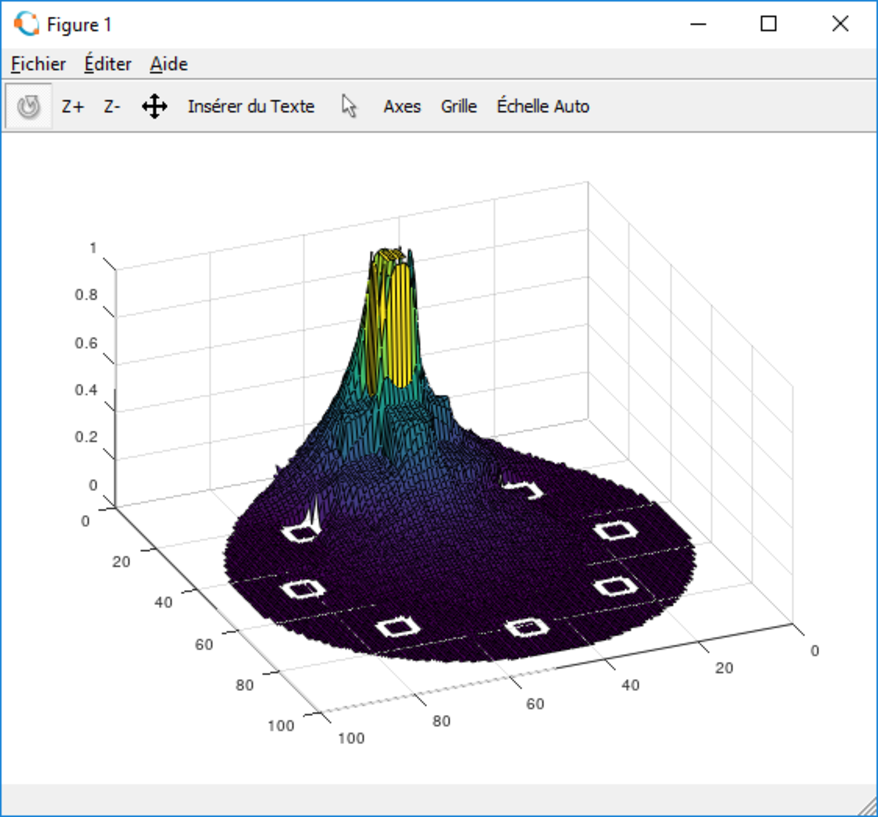
\includegraphics[scale=0.6]{plot_V_octave.pdf}
		\caption{Example of a electric potential plot in octave. }   
		\label{fig:v_octave}
	\end{figure}
	
	\begin{lstlisting}
	surf(Vfinal(:,:,100))
	\end{lstlisting}
	Only one slice of the potential can be viewed at the same time as shown in fig. XX. For a more complete visualisation, it is recommended to use Paraview software.
	First, the voltage has to be saved in a format readable by Paraview, this is done by the routine \lstinline{save_V}:
	
	\begin{lstlisting}
	save_V(Vfinal,'path\filename.csv');
	\end{lstlisting}
		\begin{figure}[!htb]
			\centering
			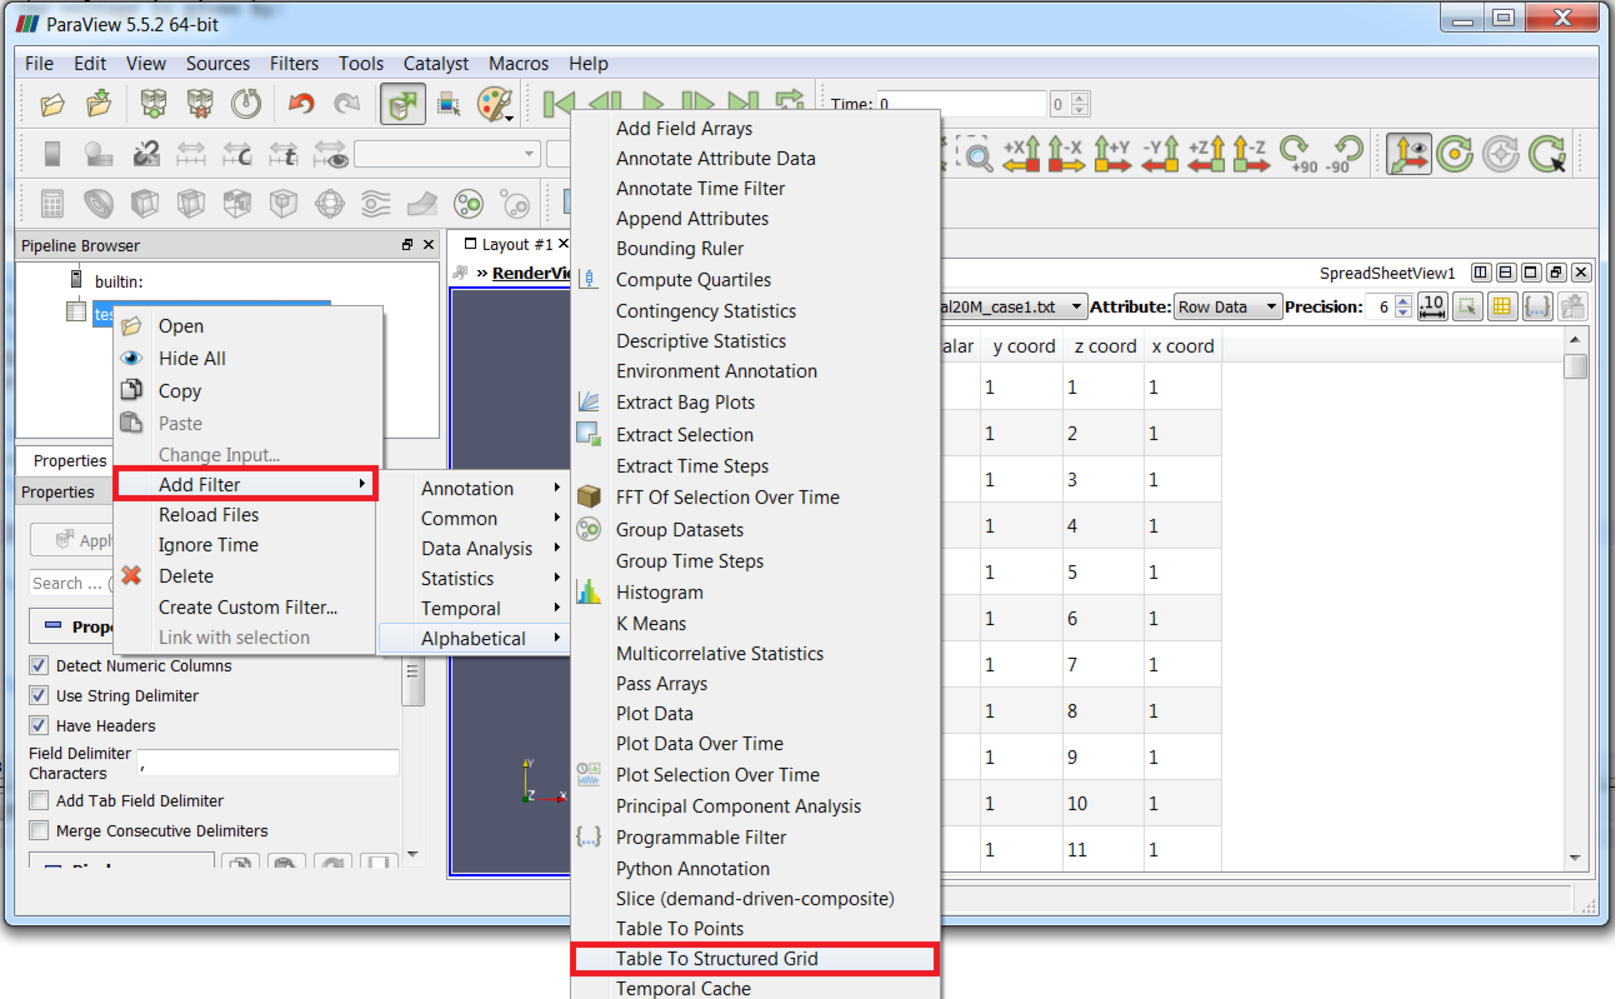
\includegraphics[scale=0.5]{paraview_config.pdf}
			\caption{Configuration of Paraview filters to plot electric potential computed by COSICAF.}   
			\label{fig:paraview_config}
		\end{figure}
	In paraview, the produced file has to be load and a "table to structured grid filter" must be applied on the data (fig.\ref{fig:paraview_config}). The filter ask to define a x,y,z column and their extent. Once every parameter is defined, a 3d plot of the electric potential is available as shown in fig.\ref{fig:v_paraview}. The representation chosen should be volume ou surface with additional filters likes "slice" or "clip".
		\begin{figure}[!htb]
			\centering
			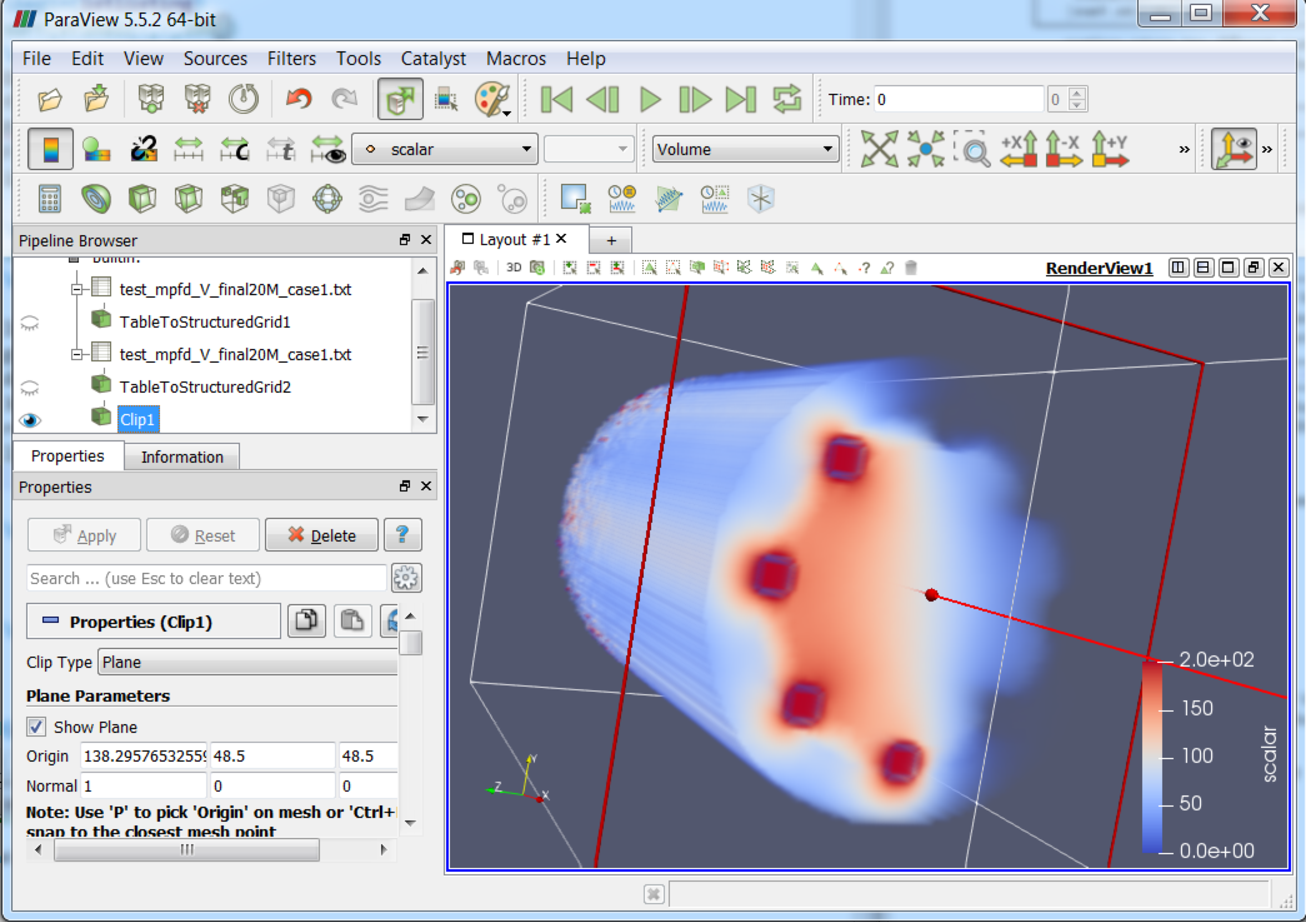
\includegraphics[scale=0.5]{paraview.pdf}
			\caption{Example of an electric potential plot in Paraview.}   
			\label{fig:v_paraview}
		\end{figure}
		
	
	\section{Function reference}
	
		\subsection{Data loading}
		
		\begin{itemize}
			\item \lstinline{function ret=load_W(obj)} This routine load the data located in \lstinline{W.dat} in COSICAF main directory. The loaded data is located in \lstinline{obj.W}, it consist in a cell array. The function return 0 if the loading was not done properly else, 1 is returned.
			
			\item \lstinline{function ret=load_molar_mass(obj)}This routine load the data located in \lstinline{molar_mass.dat} into \lstinline{obj.molar_mass}. It return 0 if the loading was not done properly.
			
			\item \lstinline{function ret=load_moderation_laws(obj)}
			\item \lstinline{function ret=load_ion_drift_velocity(obj)}
			\item \lstinline{function ret=load_elecEcorr(obj)}
		\item \lstinline{function ret=load_e_drift_velocity(obj)}
			
		\end{itemize}
		
		\subsection{Basic models}
		\begin{itemize}
		\item \lstinline{function R=range(obj,medium,mass_vol,particle)} This routine return the range (in m) of the particle in a medium. The argument are: \lstinline{medium} a string representing the target medium \lstinline{mass_vol} the volumic mass (in g/cm$^{3}$) of the targed medium and \lstinline{particle} a string representing the projectile.
		\item \lstinline{function E=moderation_law(obj,medium,mass_vol,particle,dist,approx)} This function return the energy of a heavy ion after a specified travel (in MeV). The routine takes as input \lstinline{medium} the name of the target medium, \lstinline{mass_vol}, its volumic mass (in g/cm$^{3}$). \lstinline{particle} is the name of the heavy ion, \lstinline{dist} 
		the distance travelled (in m) and \lstinline{approx} the approximation law of the moderation law.  
		\item \lstinline{function l=inverse_moderation_law(obj,medium,mass_vol,particle,E, approx)} This routine computes inverse moderation law. From the kinetic energy \lstinline{E} (in MeV) of a projectile \lstinline{particle}, it is possible to compute the distance travelled inside a medium with a \lstinline{mass_vol} volumic mass (in g/cm$^{3}$) . Depending on the approximation of the moderation law used, either inversion or a bisection method is used to compute and return the travelled distance (in m).
		\item \lstinline{function W=get_W_value(obj,material)} This routine return the W value in the specified \lstinline{material}.. 
		\item \lstinline{function Ecorr=elecE_corr(obj,medium,particle,E)}
		\item \lstinline{function vel=e_drift_velocity(obj,medium,reducedE)} The function compute the electron drift velocity in the medium specified by the \lstinline{medium} argument. The reduced electric field \lstinline{reducedE} is needed (in Td) to perform the computation. 
		
		\item \lstinline{function Er=compute_reduced_Efield(obj,E,mater,density)}
		\end{itemize}
		\subsection{Geometry related}
		\begin{itemize}
		\item \lstinline{function l=load_geometry(obj,filname)} The function open the filename specified in \lstinline{filname} and parse the geometry it contains. All the data about the problem geometry is stored as a cell array in \lstinline{obj.moderation_laws}.
		\item \lstinline{function ind=find_volume_next_to_intersection(obj,pos,direction)} This  routine find which volume is toward an intersection point. It takes as input a surface/trajectory intersection point \lstinline{pos} and a direction of propagation \lstinline{direction} to compute the next visited volume. The routine compute a new position wich is located $3e-9$ m away from the intersection point and call the \lstinline{find_volume_by_location} to retrieve the next volume. If no volume was found, an empty vector is returned. 
		\item \lstinline{function ind=find_volume_by_location(obj,pos)} This routine find in wich volume is a point located  at \lstinline{pos} coordinates. It take as input a 3 element vector representing the location of interest. The function sort each geometry volume by decreasing inclusion index and go through the sorted volumes while checking if \lstinline{pos} is included inside. If \lstinline{pos} is included in a volume, its index is returned. If no volume was found, an empty vector is returned.
		\item \lstinline{function vec=find_intersection_point(obj,volume_ind,direction,pos)} This routine find an intersection point between a volume and a heavy ion trajectory. It takes as input \lstinline{volume_ind}, the volume's index where the ion is located, \lstinline{direction} and \lstinline{pos}, 3 elements vectors representing respectively the direction of propagation and the actual position of the ion. The routine first check the possible intersection between int volume with the  \lstinline{volume_ind} index. Possible intersection are also computed with inner volumes. At last, the closest intersection point is selected and returned.
		 
		\item \lstinline{function ind=find_inner_volume(obj,volume_ind)} This routine find volumes included in the volume \lstinline{volume_ind}. If the volum contains no inner volume, an empty vector is returned.
		\item \lstinline{function draw_geometry(obj)} This function draws in 3D the geometry previously loaded in memory with \lstinline {load_geometry}.  
		\item \lstinline{function [condlim,permit,pos_voxel,pos_geom]=convert_geom_Vmcsolver(obj,dl)} This routine converts the surface geometry into a discrete one. It takes as parameter \lstinline{dl} the discretisation step and return two 3d matrix, \lstinline{condlim} and \lstinline{permit} which contain respectively the pontential boundary conditions and the permittivity. In position where no boundary condition was defined,  \lstinline{condlim} contain 1e9 values. The discretization is done by using Brensenham circle algorithm in conjunction with a flood and fill algorithm. Two 3 elements vectors are also returned the contains the location of the geometry bound origin in the discretized geometry (in matrix index) and in the surface geometry. 
		\item \lstinline{ret=draw_voxel(mat,value)} This routine perform a voxel plot of the 3d matrix \lstinline{mat} (fig.\ref{fig:voxel}). It draws only the data point with a value specified in the 1 dimension \lstinline{value} vector. Each value corresponds to a specific color on the plot. 
		
			\begin{figure}[!htb]
			\centering
			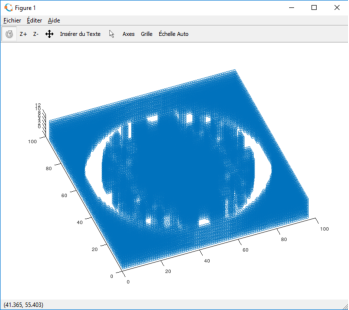
\includegraphics[scale=1.4]{voxel.pdf}
			\caption{Example of a voxel plot of the dielectric permittivity matrix. Only the relative permittivity of 1 is plotted here.}   
			\label{fig:voxel}
		\end{figure}
		
		\end{itemize}
		\subsection{Heavy ion propagation}
		\begin{itemize}
		\item \lstinline{function ret=init_heavy_particles(obj)} This routine takes the sources definition in geometry and initialize \lstinline{obj.particle_nb} particle. For each particle, its kind, its initial position and energy is set, as well as its propagation direction.
		
		\item \lstinline{function ret=propagate_one_heavy_particle(obj,part_index,approx)} The routine makes propagate the particle with the index \lstinline{part_index}. It moves the particles from volume boundary to volume boundary, computing the energy loss between each intersection with moderation laws. The moderation laws approximation are specified using the \lstinline{approx} argument. Trajectory steps are stored in \lstinline| obj.particle{3,part_index} |. The trajectory is written in the following way: energy, pos x, pos y pos z, cur vol, next vol,energy, pos x, pos y, pos z ... 
		\item \lstinline{function draw_particle_trajectory(obj, traj_ind)}
		The routine is able to compute a trajectory with the index \lstinline{traj_ind}. Be sure to have already computed the trajectory before plotting it.
		\item \lstinline{function t=compute_hion_traveling_time(obj,medium, mass_vol,particle,beg,fin,approx)} This routine compute the traveling time of an heavy ion between \lstinline{beg} length and \lstinline{fin} length (in m). \lstinline{beg} allow to start with an energy different from the heavy ion initial energy. \lstinline{medium} is a string representing a target medium with a \lstinline{mass_vol} volumic mass (in g/cm$^{3}$). \lstinline{particle} is a string representing the heavy ion of interest. Up to now, this routine is not well written and should be modified.
		
		\end{itemize}
		\subsection{Signal generation}
		\begin{itemize}
		\item \lstinline{function ret=move_charge_track(obj,signal_ind)}
		\item \lstinline{function ret=kill_ions(obj)} This routine remove all the ions from the charges generated by \lstinline{generate_charge_track}, that is to say all the element of charge positive value of charge: \lstinline{obj.charges(:,5)>0}
		\item \lstinline{function ret=kill_electrons(obj)} This routine remove all the electrons from the charges generated by \lstinline{generate_charge_track}, that is to say all the element of charge positive value of charge: \lstinline{obj.charges(:,5)<0}
		\item \lstinline{function [ret]=generate_charge_track(obj, part_index,approx)} This routine build an array stored in \lstinline{obj.charge} and store in it charged meta-particles corresponding to a ionisation track with the \lstinline{part_index} index. To generate meta-particles, the routine compute where on the trajectory it is possible to generate an ion pair (the W data is checked to see if the medium of interest has a reference). Then, this part of the trajectory is cut in \lstinline{obj.particle_nb} pieces and two charged meta-particles, one positive and one negative are created in the middle of the small trajectory pieces. Everything is stored in the \lstinline{obj.charge} array with the following format for each row: x$_p$,y$_p$, z$_p$, charge amount (in $qe$), charge sign (+1 for ions -1 for electrons, 0 for a dead meta-particle).
		\item \lstinline{function draw_charged_particles(obj, sign)}
		\end{itemize}
		\subsection{Electrostatic}
		\begin{itemize}
		\item \lstinline{function E=compute_E_from_mc_V(obj,x,V,pos_voxel,pos_geom,dl)} This routine computes the electric field  (in V/m) from a electric potential matrix by using a centred finite difference for gradient approximation. Because of the technique used, it is mandatory to have a smooth electric potential since the approximate derivative increase the noise. The routine takes as input \lstinline{x} the position where the electric field is computed, \lstinline{V} the potential 3d matrix, \lstinline{pos_voxel} and \lstinline{pos_geom} the location of the geometry origin respectively in voxel unit and in meter and \lstinline{dl} the discretization step. 
		\item \lstinline{function ret=load_geometry_electrostat_dat(obj,filname)} This function load the data related to electrostatic for the geometry already in memory.
		\item \lstinline{function [V,nbpass]=solve_mc_V(obj,condlim,permit,iter)} 
		\end{itemize}
		
		
		
	\section{Licence} 
	
	
	
\end{document}